\documentclass[12pt,letterpaper]{article}

\usepackage{amsmath, amsthm}
\usepackage{graphicx,hyperref}
\usepackage[comma,sort&compress]{natbib}
\usepackage{docmute}
\usepackage{subcaption, multirow, morefloats}
\usepackage{wrapfig}

\frenchspacing

\captionsetup[subfigure]{position = top, labelfont = bf, textfont = normalfont, singlelinecheck = off, justification = raggedright}

\begin{document}
\section{Results}
% \hat{R} values indicate approximate convergence of all chains for all parameter estimates.
% The table is for key parameters of interest.
% Given these estimated parameter values, how well does my model fit?
%   Deviance residuals indicate the major problem is over estimation of duration.
%   However, there residuals are not oddly shaped, approximately good fit for the mean.
%   Comparison of empirical survival to 100 estimates shows pretty good congruence.
%   Corroborated with comparison of empirical point estimates with simulated distributions.
% The model seems a pretty good descriptor of expected duration.

With all marginal posterior estimates having converged (\(\hat{R} < 1.1\)) it is possible be examine the quality of model fit (Table \ref{tab:post_sum}). If the model is an adequate descriptor of the observed data, then relatively confident inference can be made \citep{Gelman2013d}.

Visual examination of the deviance residuals from twelve different sets of posterior predictive simulations indicates few systematic problems (Fig. \ref{fig:ppc_res}). The only concern is that the residuals are slightly skewed, however this bias appears very small. This is confirmed by comparing the K-M estimate of the empirical survival function to 100 estimated survival functions from posterior simulations (Fig. \ref{fig:ppc_surv}).

Comparisons of the observed 25th, 50th, 75th quantiles, and mean durations to the results from the posterior predictive simulations indicate adequate model fit (Fig. \ref{fig:ppc_quant}). Because all the different posterior predictive checks seem to agree, the inferred model appears adequate at capturing the observed variation.

% Interpretation of parameter estimates.
%   Diet and locomotor categories and probability state X lives longer than state Y.
%   Occupancy has largest effect, as expected given how often it has been identified.
%   Mass has weakly positive effect on duration. 
%   Cohort
%     Evidence of weak effect of younger cohorts surviving longer than older cohorts.
%     However, effect has low overall variance, indicating cohorts are mostly similar.
%   Phylogeny
%     Non-zero effect, though small. Probably why ``phylo signal'' not found.
%     Slightly greater overall variance than cohort
%   VPC
%     Individual species variance is largest source of unexplained variance.
%     cohort >= phylo
%     However, cohort + phylo approx. 20\% of the unexplained variance.
%     Not ignorable effects.

Given that the model appears adequate, it is possible to interpret the parameter estimates with some degree of confidence. The estimates for diet and locomotor categories were inferred as contrasts between the intercept and one of the \(k - 1\) other states (Table \ref{tab:post_sum}). In order to interpret these estimates, I compared the differences between each of the different states to get an estimate of whether either of two traits was associated with a greater mean duration or not. This was done for all pairwise comparisons for diet and locomotor category separately (Fig. \ref{fig:trait_est}).

Dietary category has a large amount of variation in the pairwise differences of the effect on expected duration (Fig. \ref{subfig:loco}). Carnivory appears to be associated with a greater expected duration than herbivory or insectivory, while approximately equal to or less than the expected duration of an omnivore. Omnivory is associated with greater expected duration than either herbivory or insectivory. Finally, herbivory and insectivory are associated with approximately equal effects on expected duration.

For locomotor category, arboreality appears to be associated with a lower expected duration than either scansoriality or a ground dwelling life habit (Fig. \ref{subfig:diet}). Scansoriality and a ground dwelling life habit have approximately equal expected durations. % percentile differences.

The effects of both body size and bioprovince occupancy on expected duration are best interpreted from estimates from the model fit standardized data (Fig. \ref{fig:eff_other}). Of all the traits of interest, bioprovince occupancy has the largest effect size with larger occupancy associated with a longer expected duration. Body size has a very small, near zero effect on expected duration, similar to the lack of relationship between body size and generic duration \citep{Tomiya2013}.

The estimates for the individual cohort effects show a weak pattern of increased extinction risk in older Cenozoic cohorts and decreased extinction risk in younger cohorts (Fig. \ref{fig:eff_cohort}). However, this pattern is not very strong as there is a large amount of variation, particularity for older cohorts. For example, note the two cohorts between 50 and 55 My that have a much lower extinction risk than other cohorts of similar age.

Because the estimate of the Weibull shape parameter, \(\alpha\), is greater than 1 extinction risk is expected to increase with taxon age (Table \ref{tab:post_sum}). The estimate of \(\alpha\) is also rather tightly constrained, having a small posterior standard deviation. \(\alpha\) is related to the strength of time on extinction risk and is a key parameter in the hazard function \(h(t)\), calculated for a Weibull distribution as
\begin{equation}
  h(t) = \frac{\alpha}{\sigma}\left(\frac{t}{\sigma}\right)^{\alpha - 1}.
\end{equation}
\(h(t)\) can be interpreted as the rate, or approximate probability, of an individual of age \(t\) going extinct. As the value of \(\alpha\) is between 1 and 1.5, extinction risk for a given species will only gradually increase with age (Fig. \ref{fig:haz}). 

% variance partitioning coefficient
Of the three sources of variance present in the model, variation in individual species accounts for approximately 70\% of observed variance (Fig. \ref{fig:vpc}). Both cohort and phylogenetic effects account for the other 30\% of the observed variance. Both of these factors are related to some aspect of the relationship between taxa, either temporal and through shared evolutionary history. While both of these effects are the source of approximately 15\% of observed variance individually, the total combined effect of these factors indicates that neither can be ignored. For example, \citet{Housworth2004} state that when phylogenetic heritability is greater than 0, phylogenetic effect cannot be ignored. As \(VPC_{phylo}\) is equivalent to phylogenetic heritability and is greater than 0, the effect of shared evolutionary history on duration is non-ignorable.

The low amount of variance of phylogenetic effect estimated from the model (Table \ref{tab:post_sum}) may explain previously found lack of ``significant phylogenetic signal'' in generic duration \citep{Tomiya2013}.


% latex table generated in R 3.1.2 by xtable 1.7-4 package
% Thu Jan  8 17:45:30 2015
\begin{table}[c]
  \centering
  \begin{tabular}{rrrrrrrrr}
    & mean & sd & 2.5\% & 25\% & 50\% & 75\% & 97.5\% & \(\hat{R}\) \\ 
    \hline
    alpha & 1.29 & 0.03 & 1.23 & 1.27 & 1.29 & 1.31 & 1.36 & 1.00 \\ 
    intercept & -0.78 & 0.14 & -1.05 & -0.87 & -0.78 & -0.68 & -0.51 & 1.00 \\ 
    logit(occupancy) & -0.53 & 0.08 & -0.69 & -0.59 & -0.53 & -0.48 & -0.38 & 1.00 \\ 
    log(size) & -0.05 & 0.05 & -0.14 & -0.08 & -0.05 & -0.01 & 0.05 & 1.00 \\ 
    ground dwelling & -0.28 & 0.10 & -0.47 & -0.34 & -0.28 & -0.21 & -0.09 & 1.00 \\ 
    scansorial & -0.22 & 0.11 & -0.43 & -0.29 & -0.22 & -0.14 & -0.00 & 1.00 \\ 
    herbivore & 0.09 & 0.09 & -0.09 & 0.03 & 0.09 & 0.14 & 0.27 & 1.00 \\ 
    insectivore & 0.10 & 0.11 & -0.11 & 0.03 & 0.10 & 0.17 & 0.31 & 1.00 \\ 
    omnivore & -0.12 & 0.11 & -0.33 & -0.19 & -0.12 & -0.05 & 0.09 & 1.00 \\ 
    \hline
    sd cohort & 0.33 & 0.06 & 0.23 & 0.29 & 0.33 & 0.37 & 0.48 & 1.00 \\ 
    sd phylogeny & 0.11 & 0.05 & 0.03 & 0.07 & 0.10 & 0.14 & 0.23 & 1.03 \\ 
    \hline
  \end{tabular}
  \caption{Marginal posterior estimates for the praameters of interested based on 1000 posterior samples. The intercept can be interpreted as the estimate for the mean observed species. The other values are the effect of a trait on the expected species duration as expressed as deviation from the mean. The categorical variables are binary index variables where an observation is of that category or not. \(\hat{R}\) values of less than 1.1 indicate approximate chain convergence for the posterior samples.}
  \label{tab:post_sum}
\end{table}


\begin{figure}[ht]
  \centering
  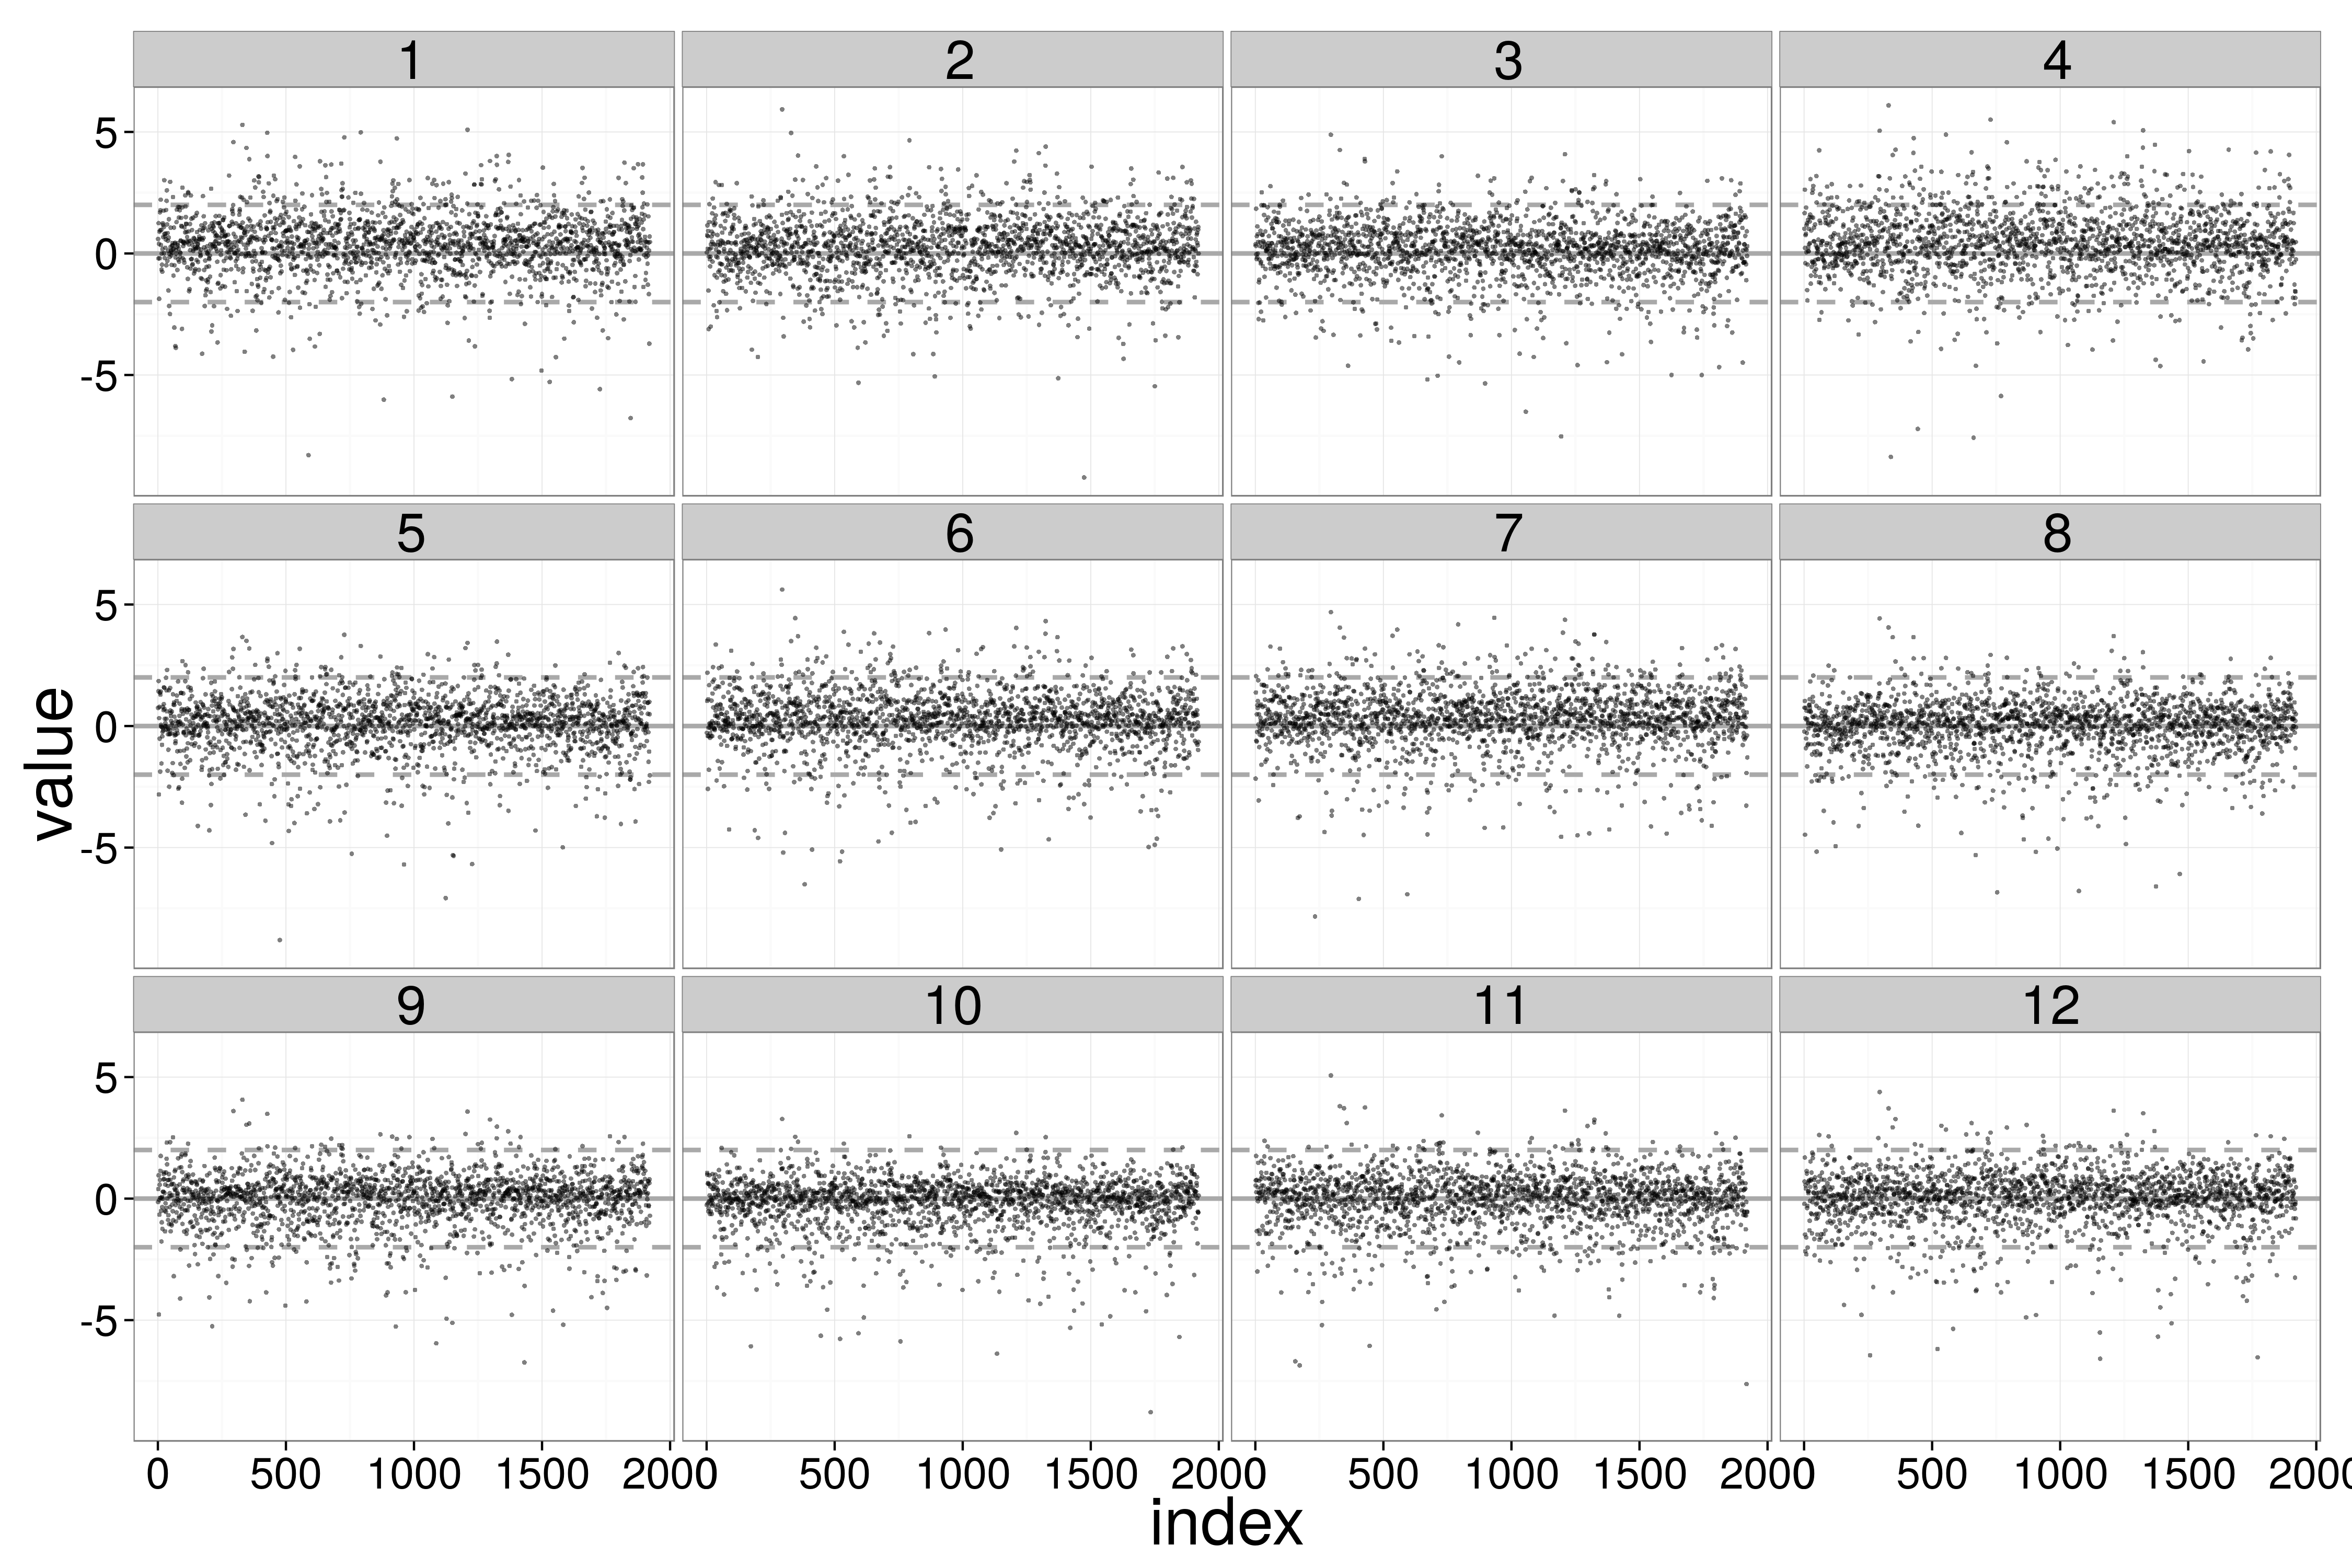
\includegraphics[height = 0.5\textheight, width = \textwidth, keepaspectratio = true]{figure/residual_plot}
  \caption{Deviance residuals from the fitted survival model. Each graph depicts the residuals from single draws from the posteriors distributions of all estimated parameters. Positive values indicate an under estimate of the observed duration, while negative values indicate an over estimate of the observed duration. Twelve difference examples are provided here to indicate the lack of individual observation based biases.}
  \label{fig:ppc_res}
\end{figure}

\begin{figure}[ht]
  \centering
  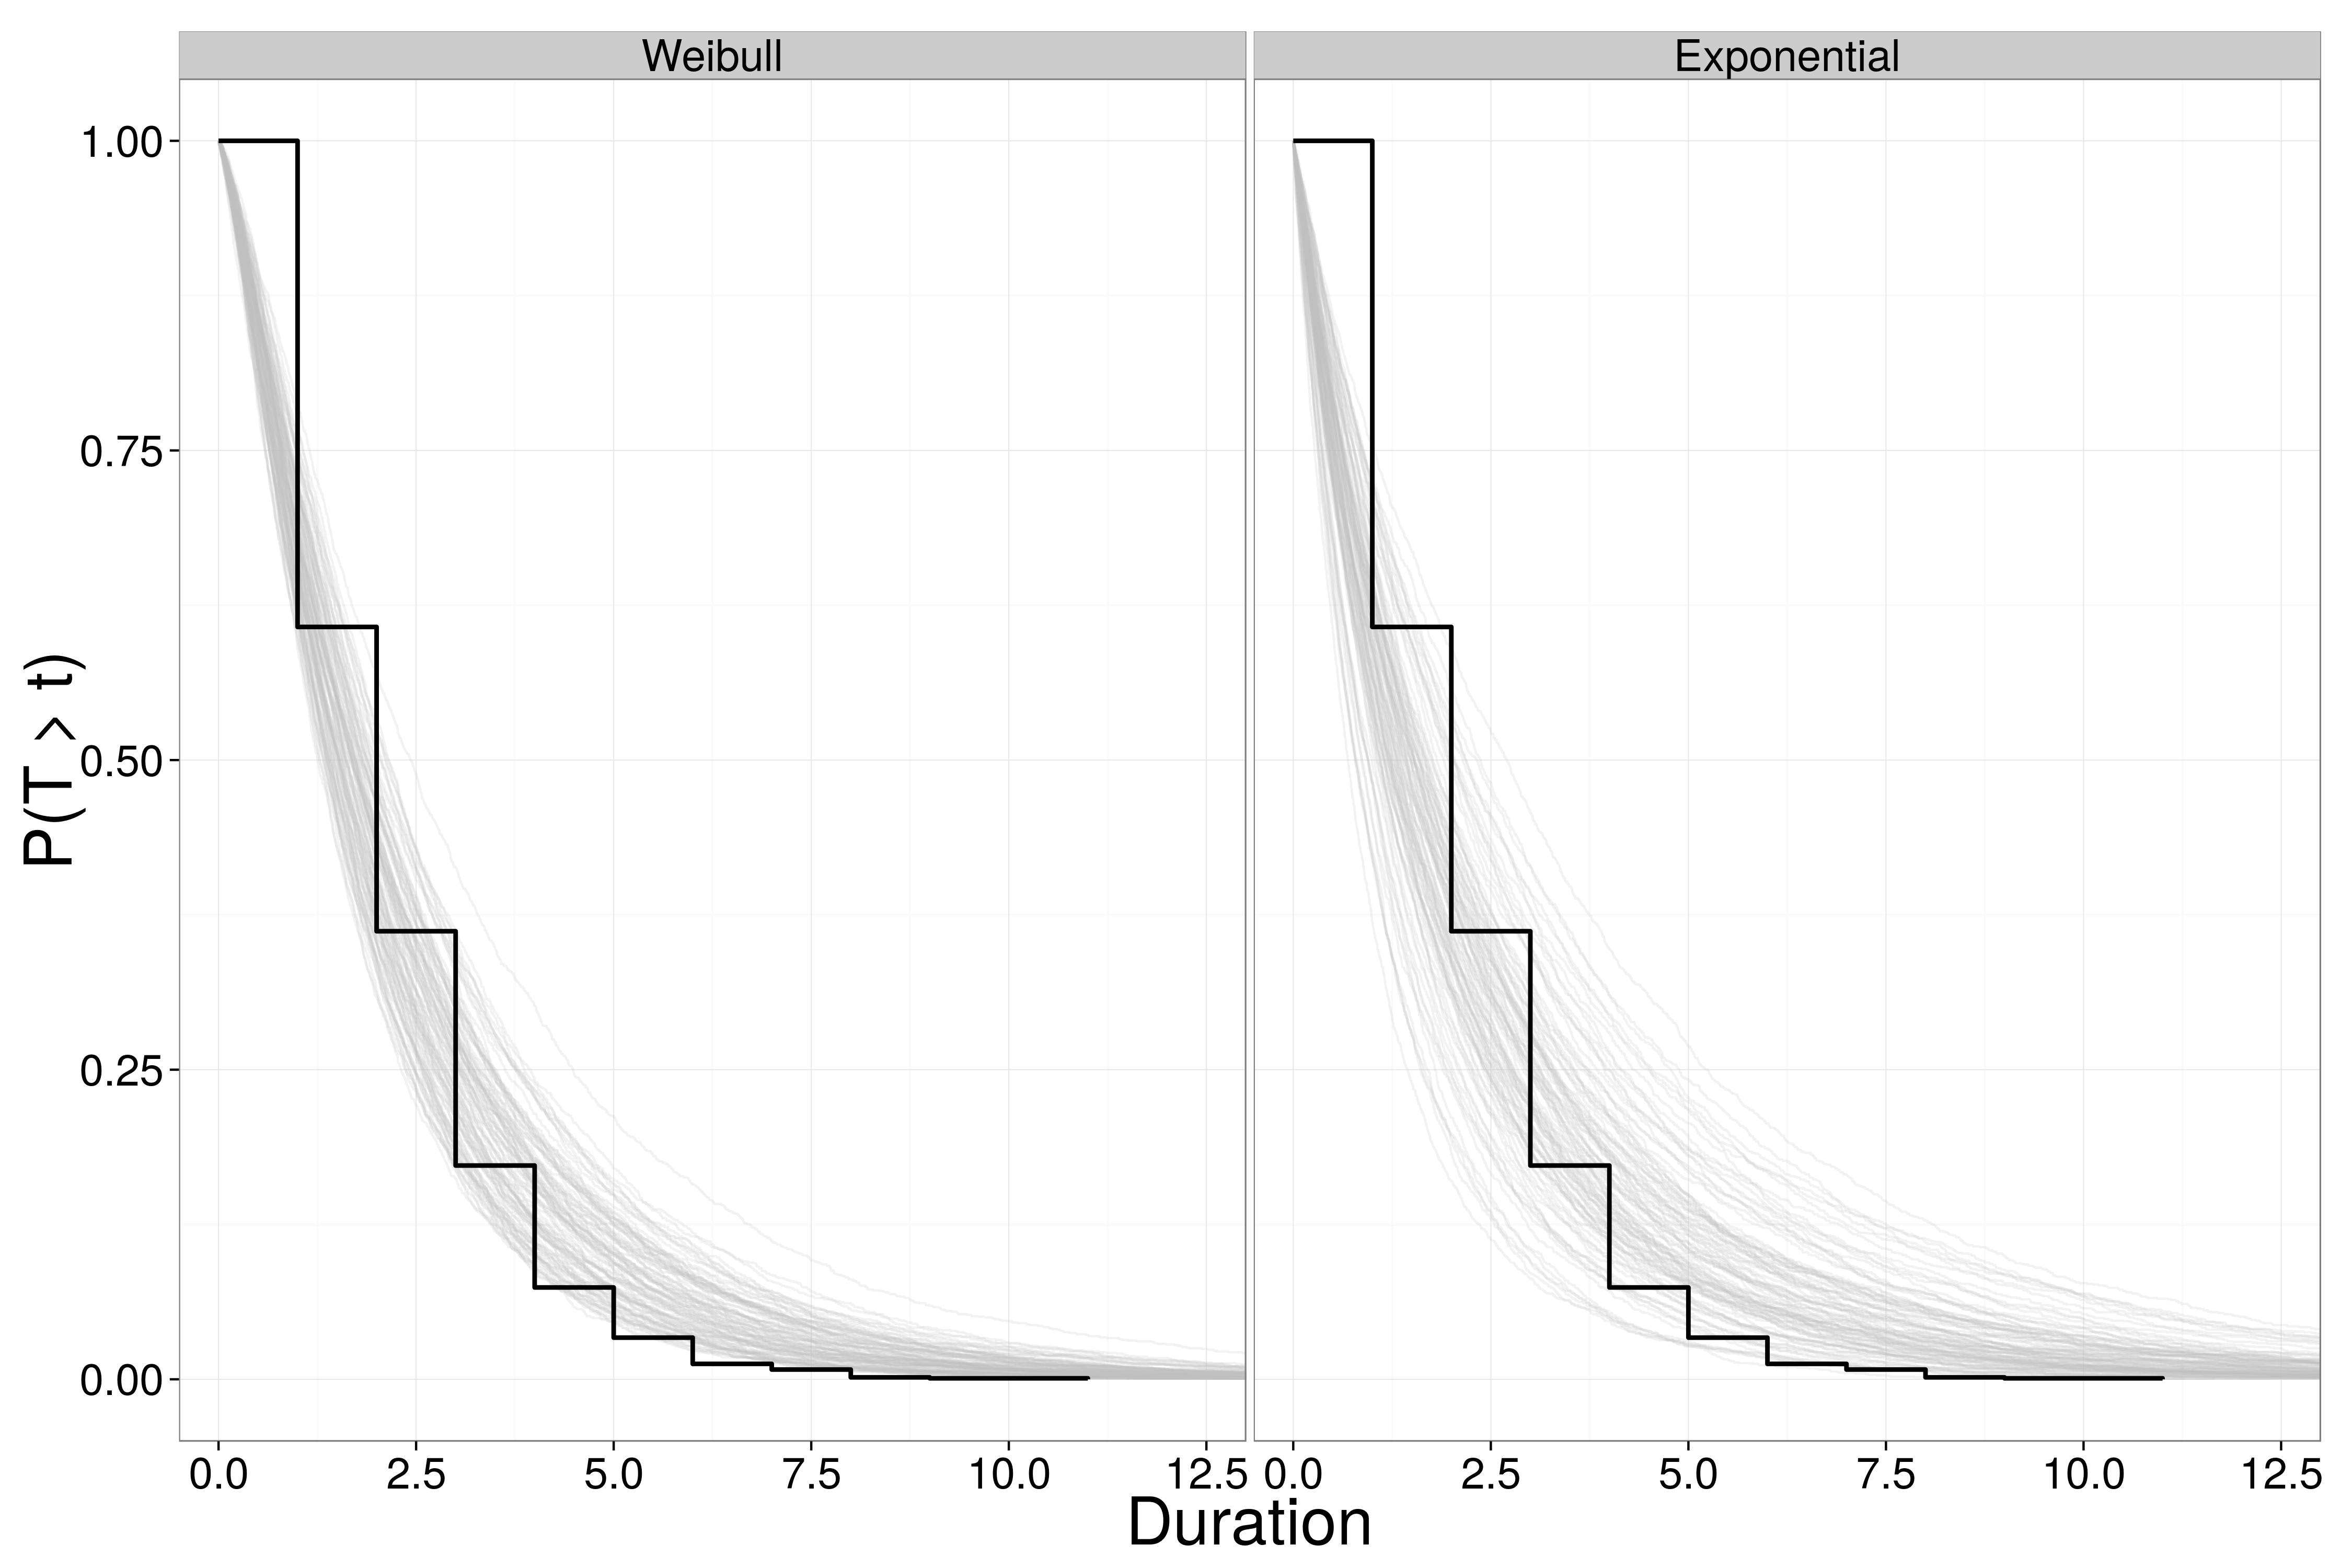
\includegraphics[height = 0.5\textheight, width = \textwidth, keepaspectratio = true]{figure/survival_function}
  \caption{Comparison between K-M estimate of survival function (black) from the observed versus K-M estimates from 100 simulated data sets using the fitted model (dark grey). Simulated data sets were generated by drawing parameter values randomly from their estimated posteriors and using the observed covariate information to estimate durations for all the observed species. On the left are the results from the full survival model (Fig. \ref{fig:model_diagram}), while on the right are the results from a simplified model where duration follows an exponential distribution and there is no phylogenetic effect.}
  \label{fig:ppc_surv}
\end{figure}

\begin{figure}[ht]
  \centering
  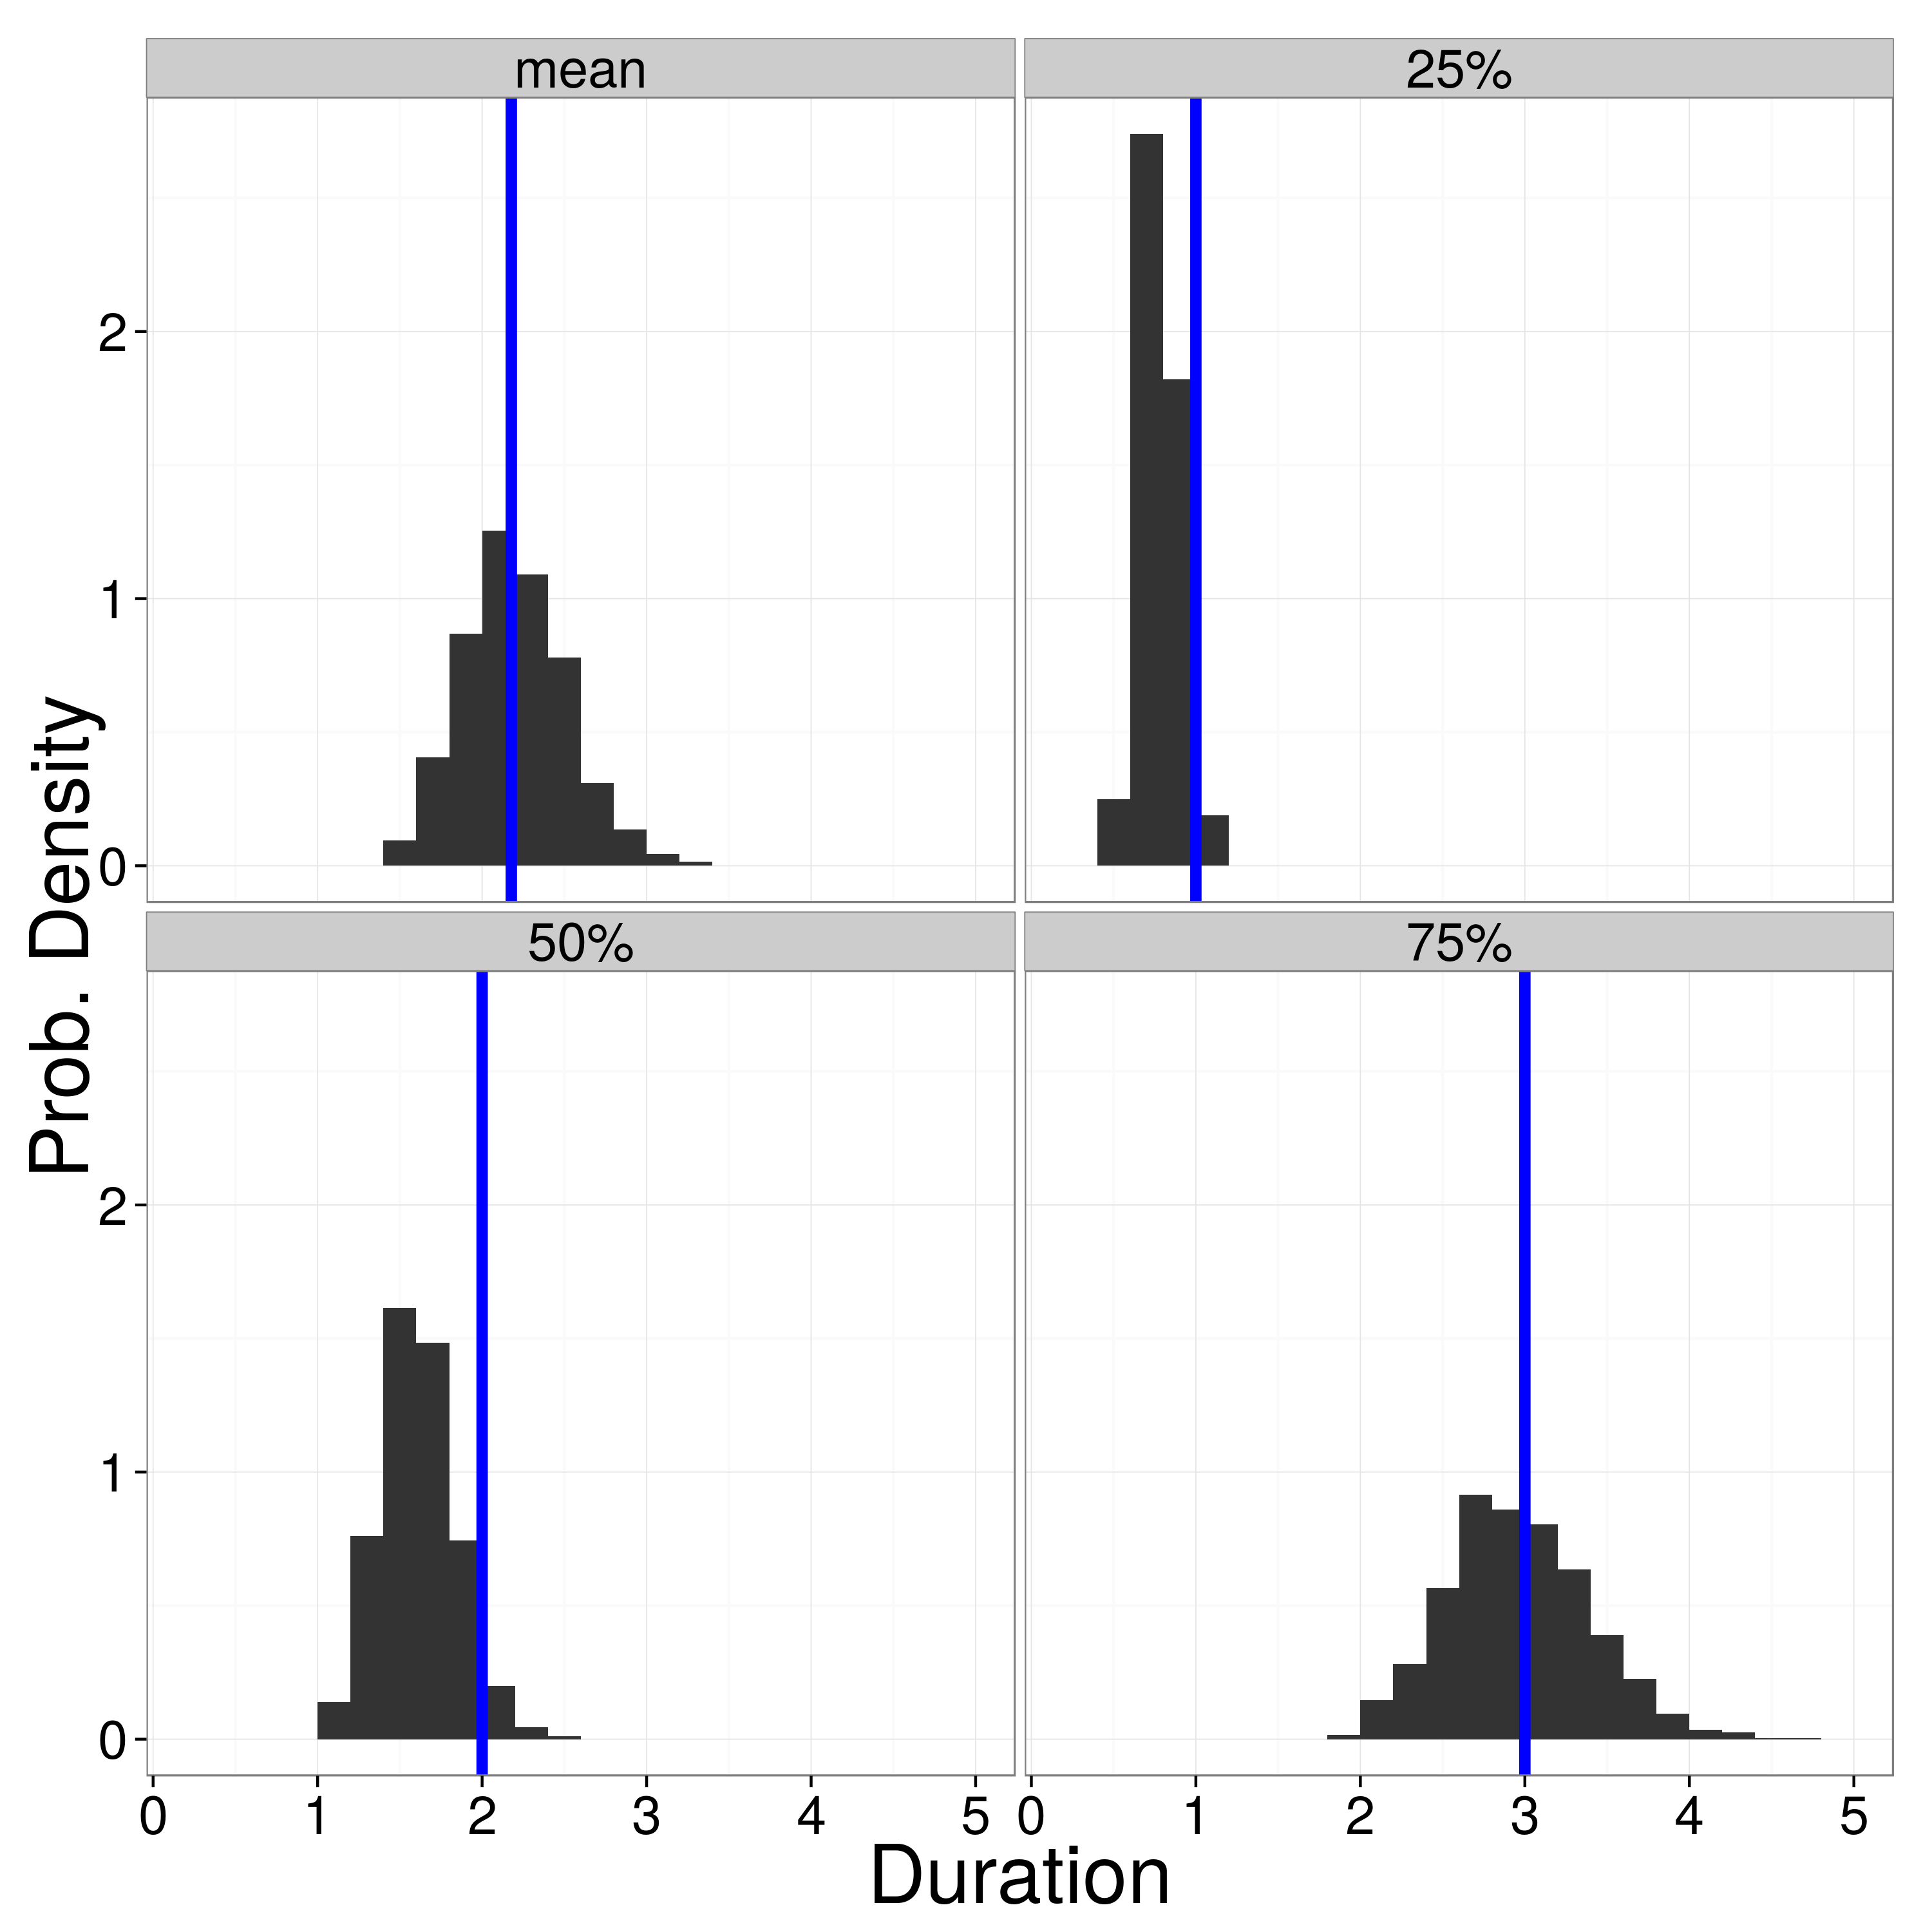
\includegraphics[height = 0.5\textheight, width = \textwidth, keepaspectratio = true]{figure/quant_ppc}
  \caption{The results of additional posterior predictive checks for four summaries of the observed durations, as labeled. Blue vertical indicate the observed value. None of the observed are significantly different from the posterior predictive distributions.}
  \label{fig:ppc_quant}
\end{figure}

\begin{figure}[ht]
  \centering
  \begin{subfigure}[b]{0.4\textwidth}
    \caption{}
    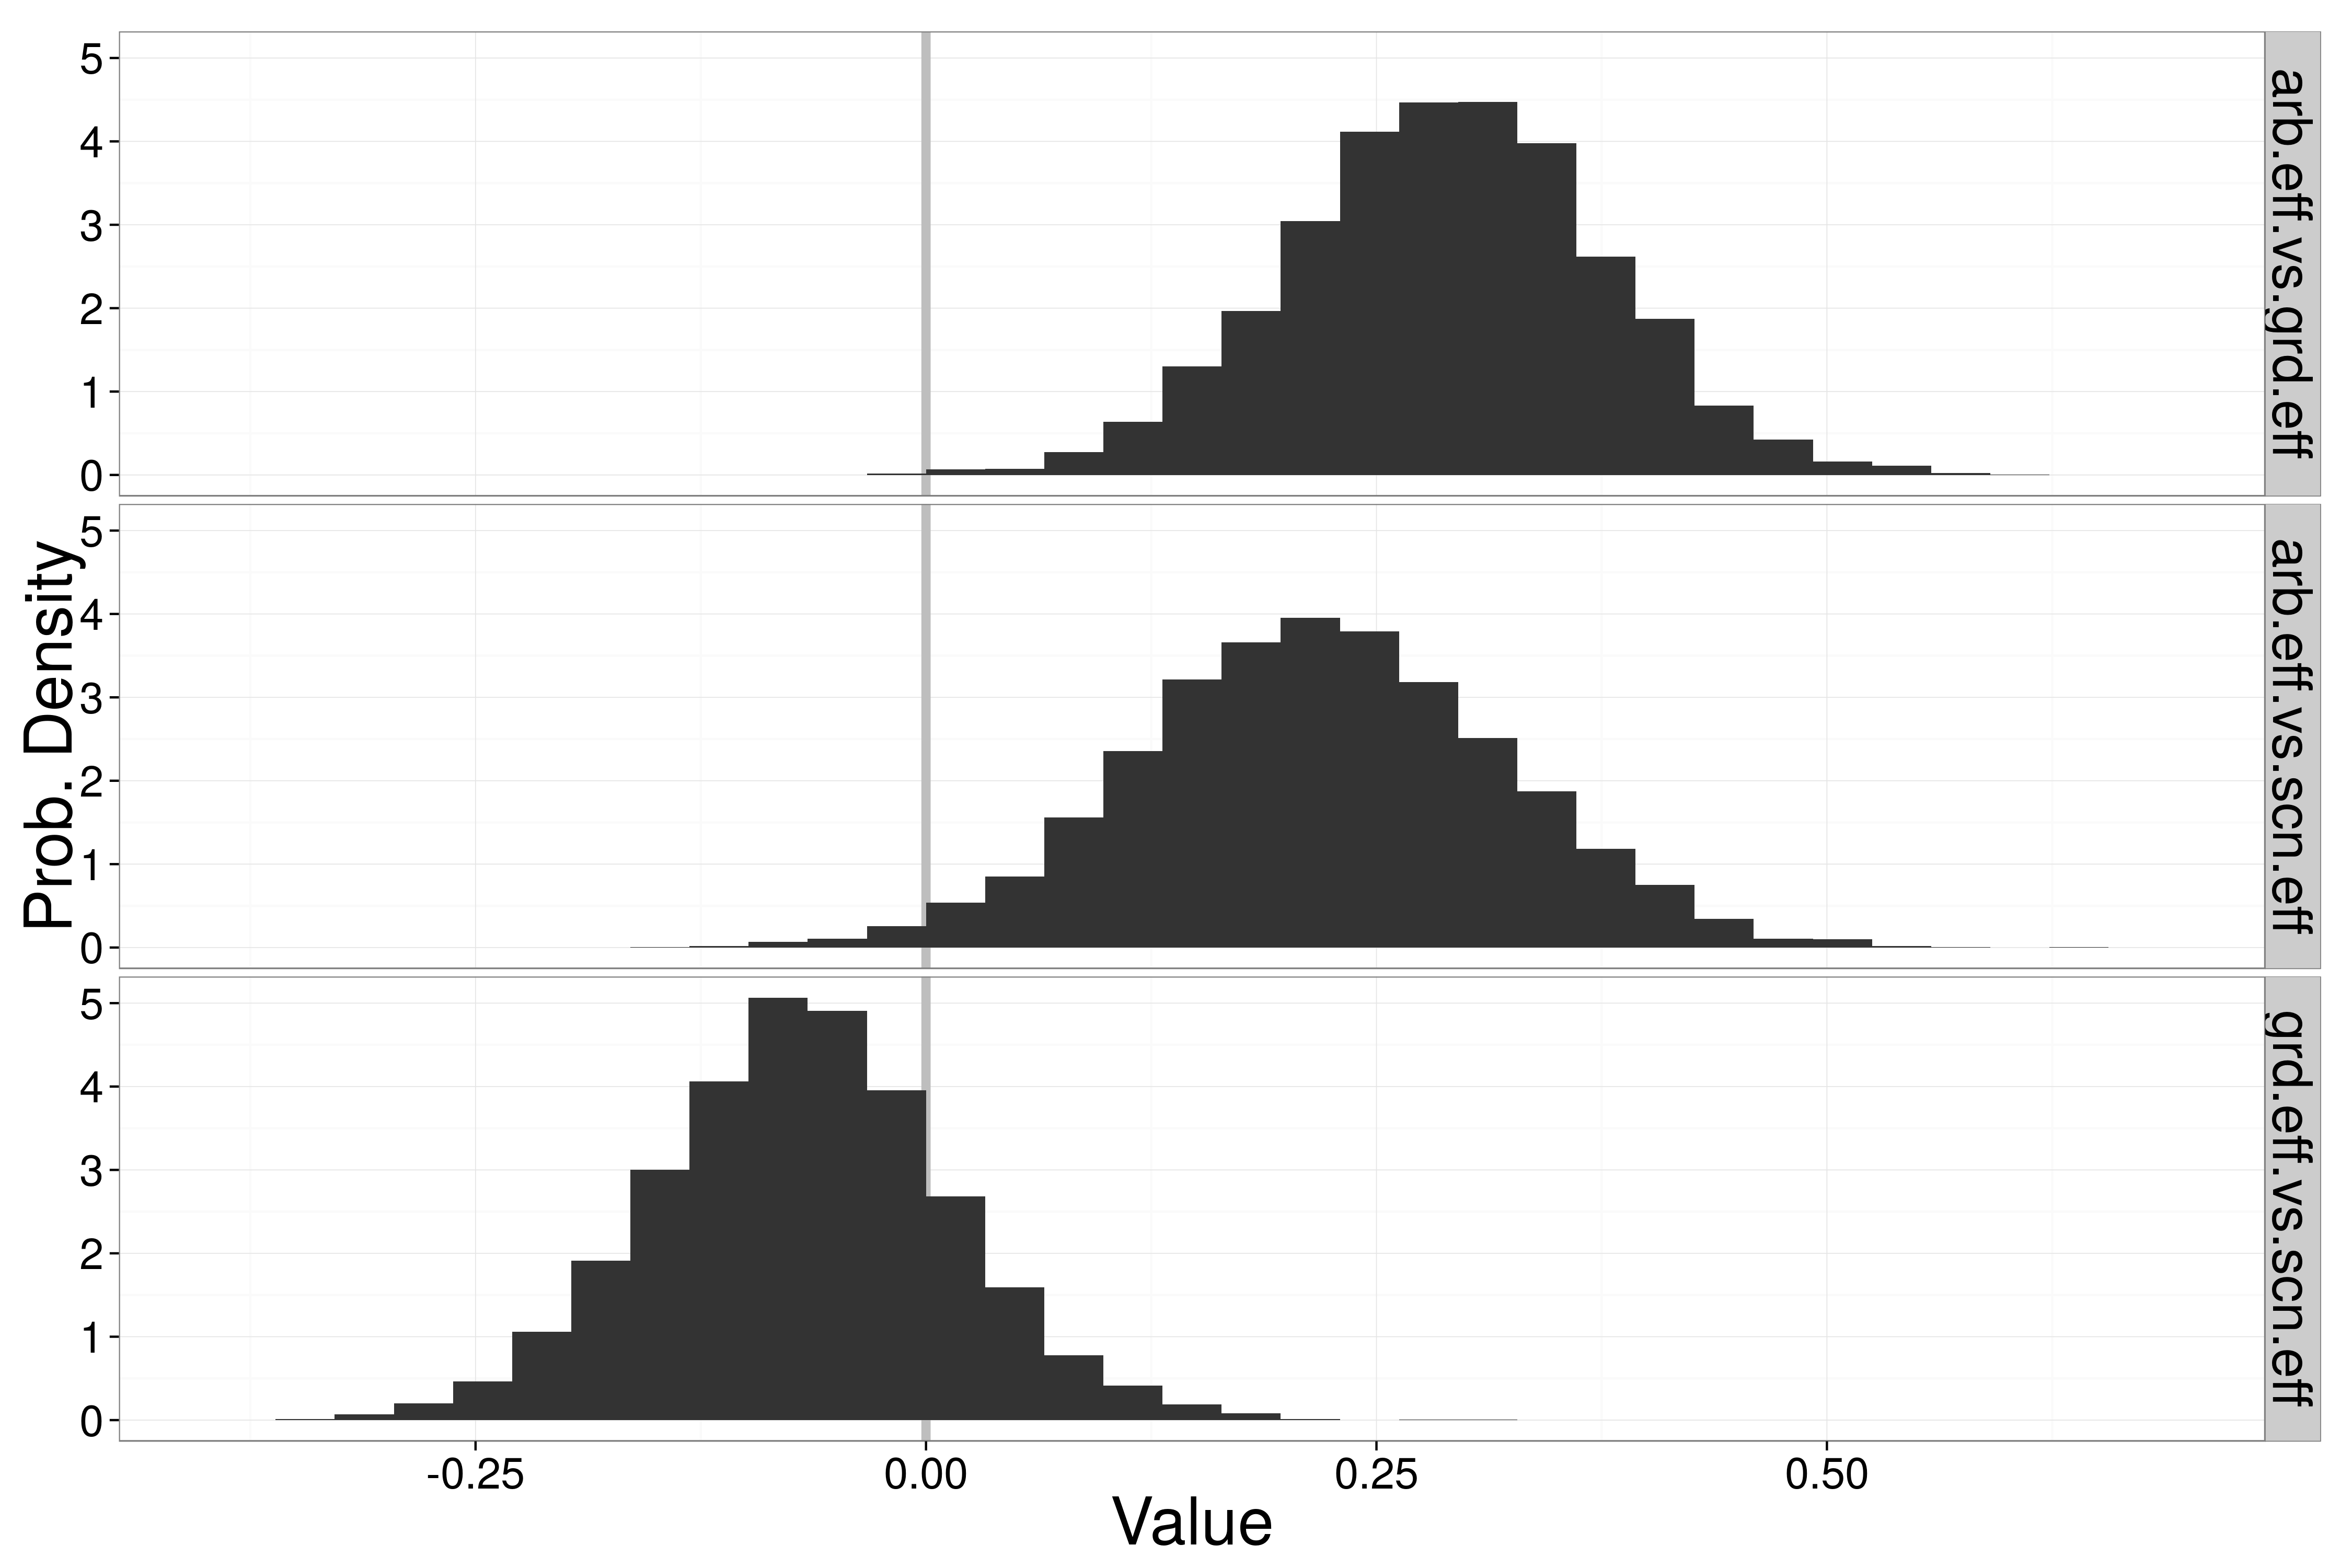
\includegraphics[height = 0.5\textheight, width = \textwidth, keepaspectratio = true]{figure/loco_diff_est}
    \label{subfig:loco}
  \end{subfigure}
  \begin{subfigure}[b]{0.4\textwidth}
    \caption{}
    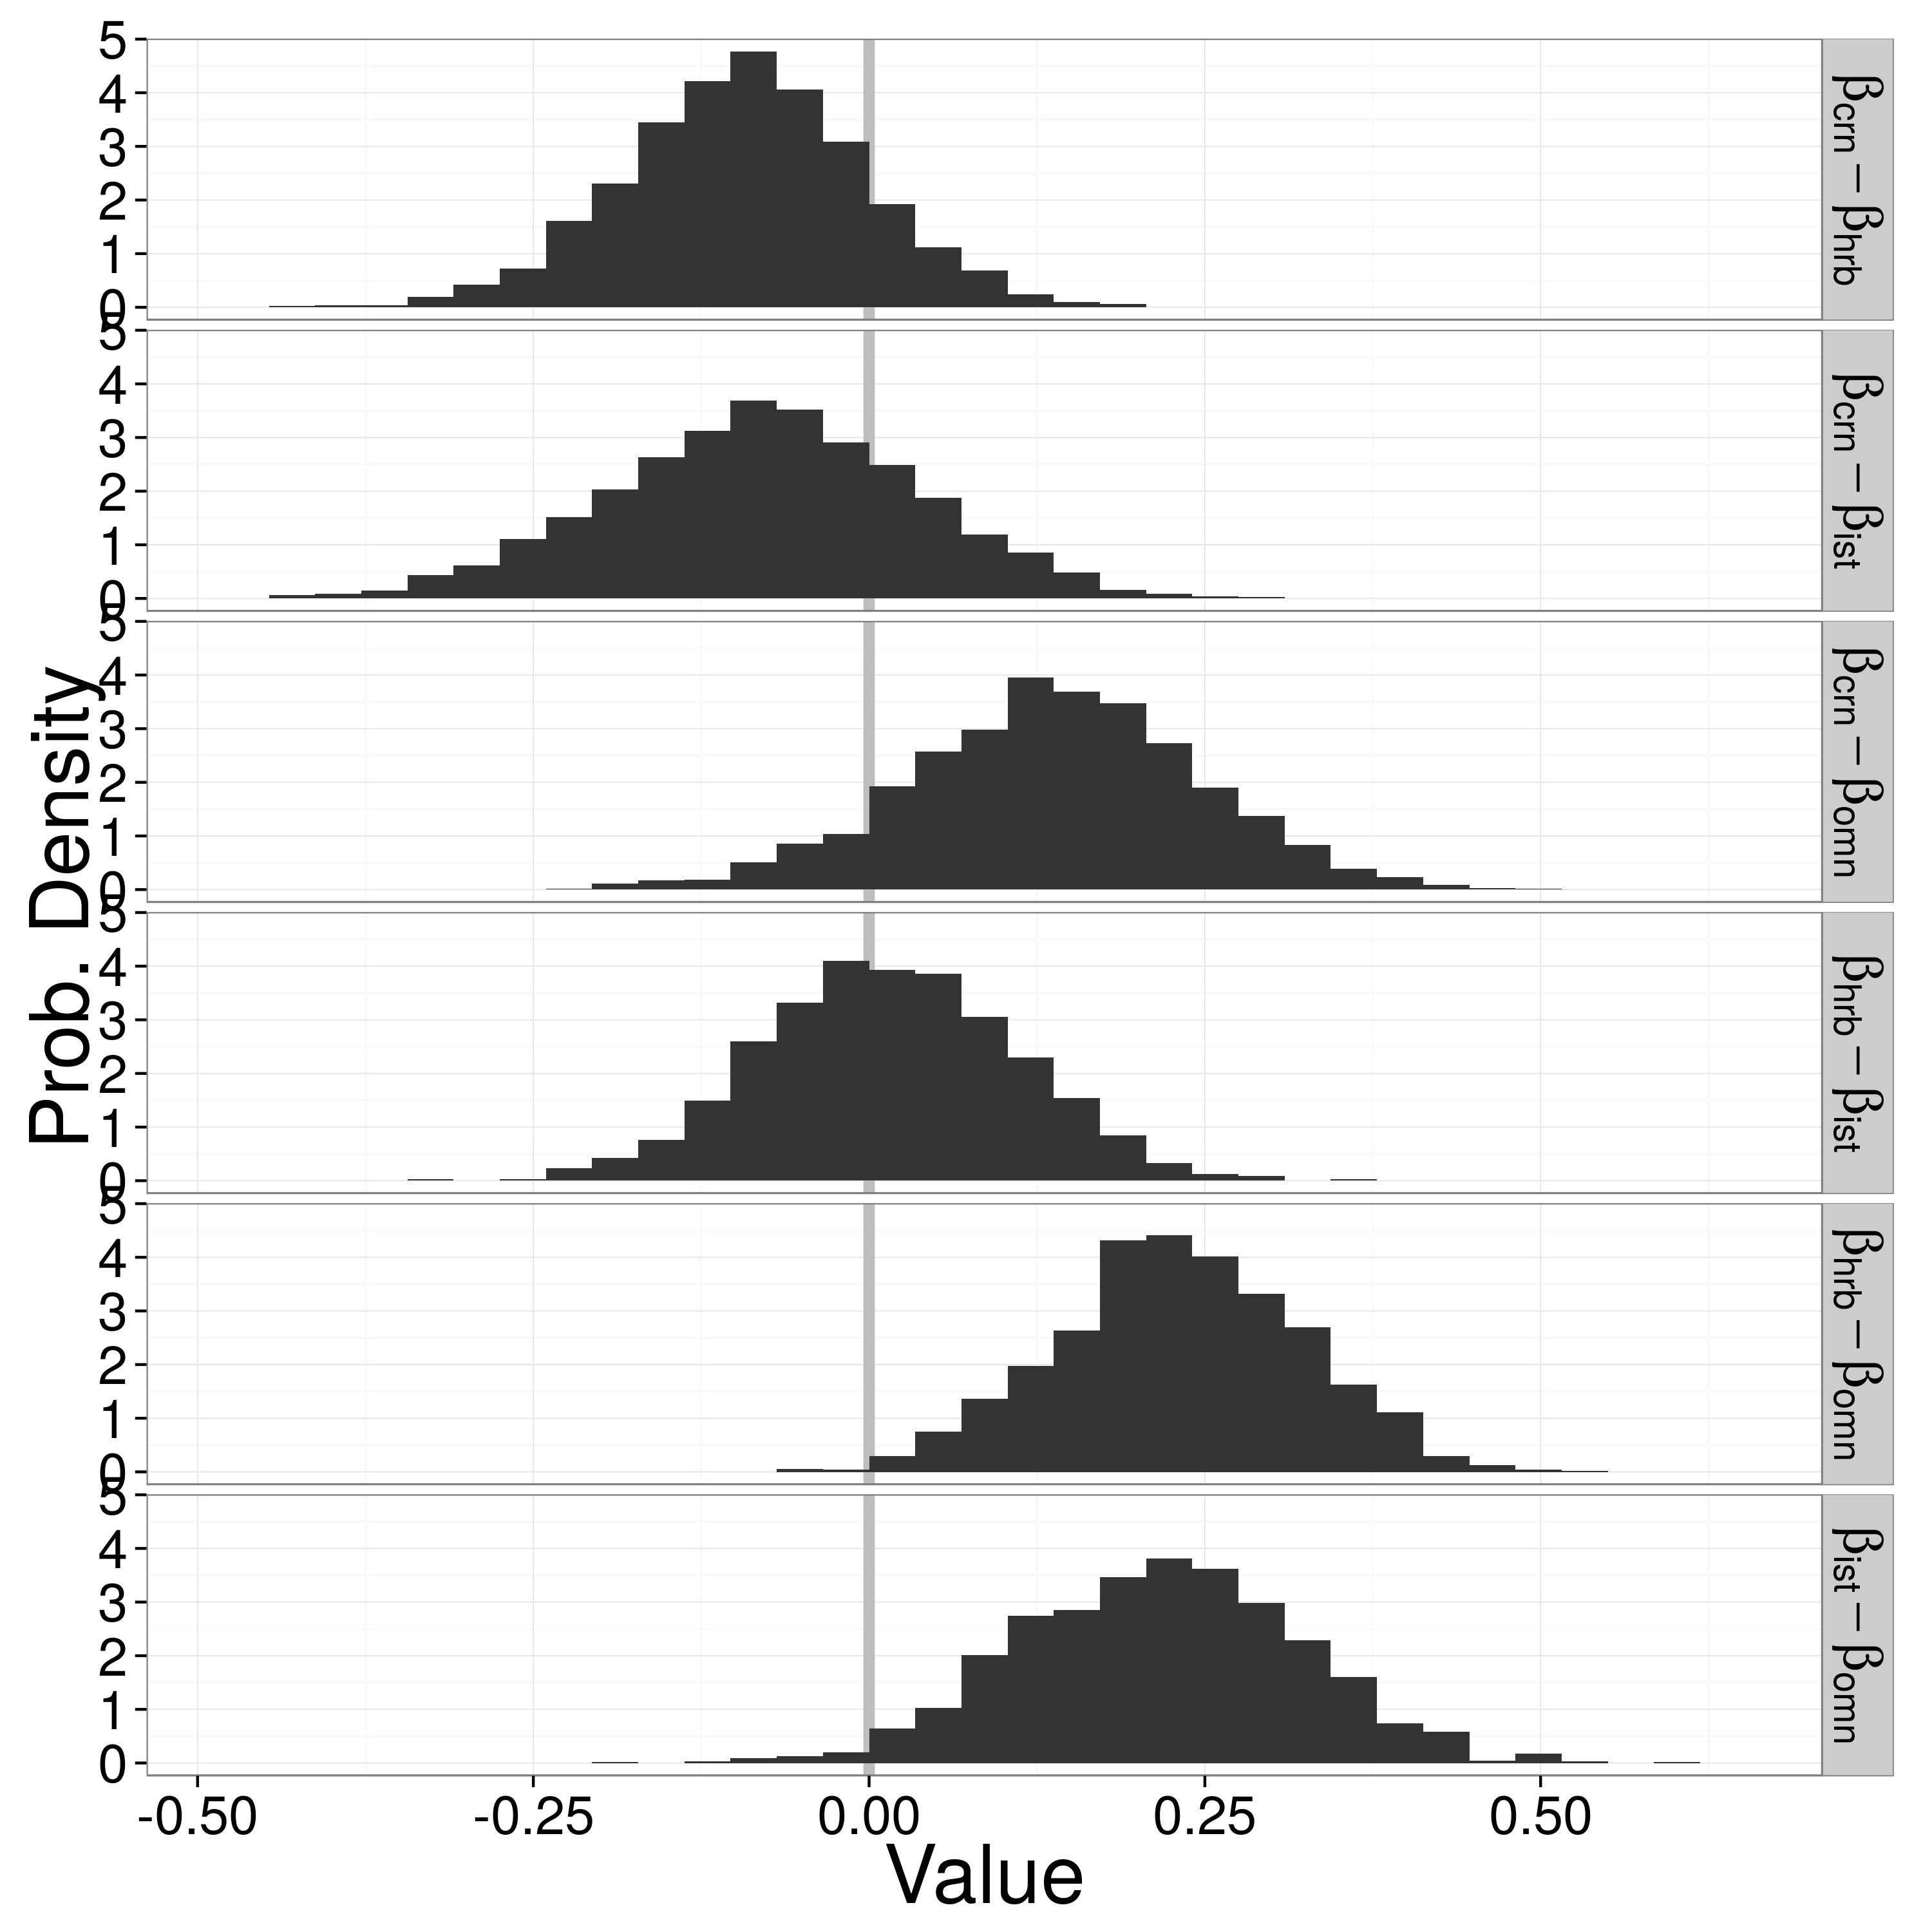
\includegraphics[height = 0.5\textheight, width = \textwidth, keepaspectratio = true]{figure/diet_diff_est}
    \label{subfig:diet}
  \end{subfigure}
  \caption{Pairwise differences in effect of the locomotor (\subref{subfig:loco}) and dietary categories (\subref{subfig:diet}) on expected duration from 1000 samples from the posterior distribution. Comparisons of locomotor categories, from top to bottom (\subref{subfig:loco}), are: arboreal versus ground dwelling, arboreal versus scansorial, and ground dwelling versus scansorial. For dietary category, from top to bottom (\subref{subfig:diet}): carnivore versus herbivore, carnivore versus insectivore, carnivore versus omnivore, herbivore versus insectivore, herbivore versus omnivore, and insectivore versus omnivore. Values to the left indicate that the first category is expected to have a greater duration than the second, while values to the right indicate that the first category is expected to have a shorter duration.}
  \label{fig:trait_est}
\end{figure}

\begin{figure}[ht]
  \centering
  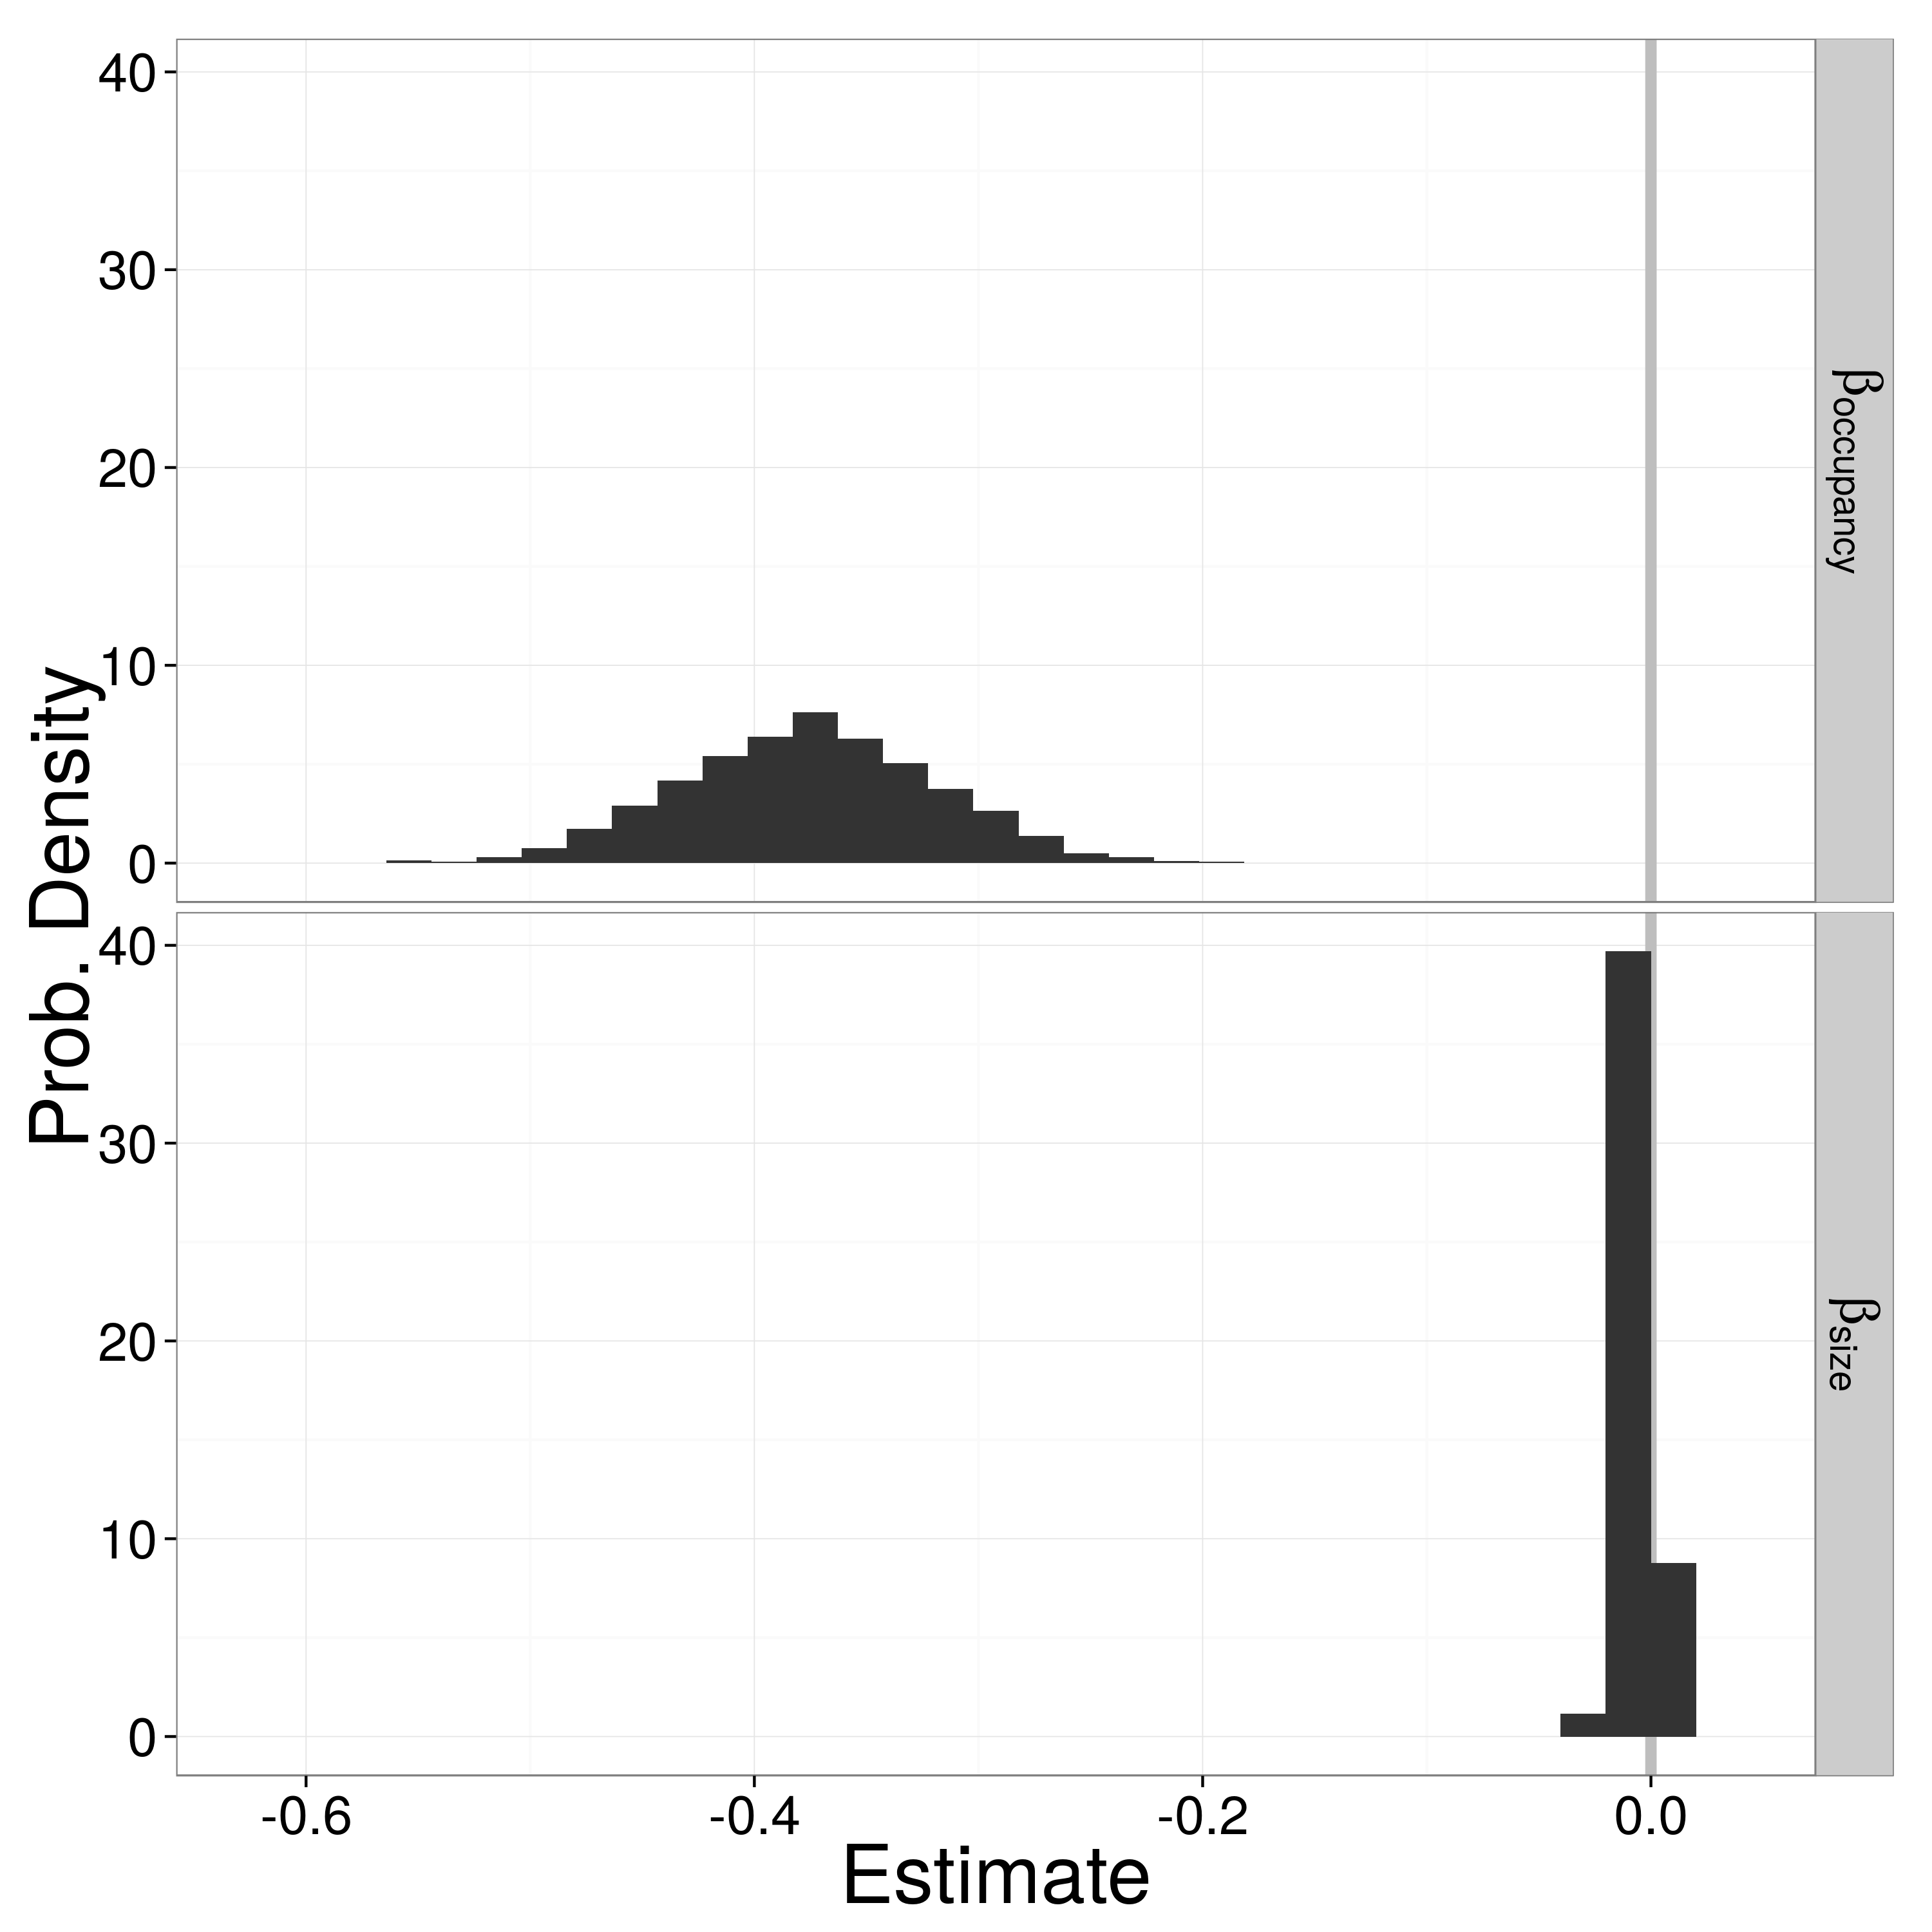
\includegraphics[height = 0.5\textheight, width = \textwidth, keepaspectratio = true]{figure/other_est}
  \caption{}
  \label{fig:eff_other}
\end{figure}

\begin{figure}[ht]
  \centering
  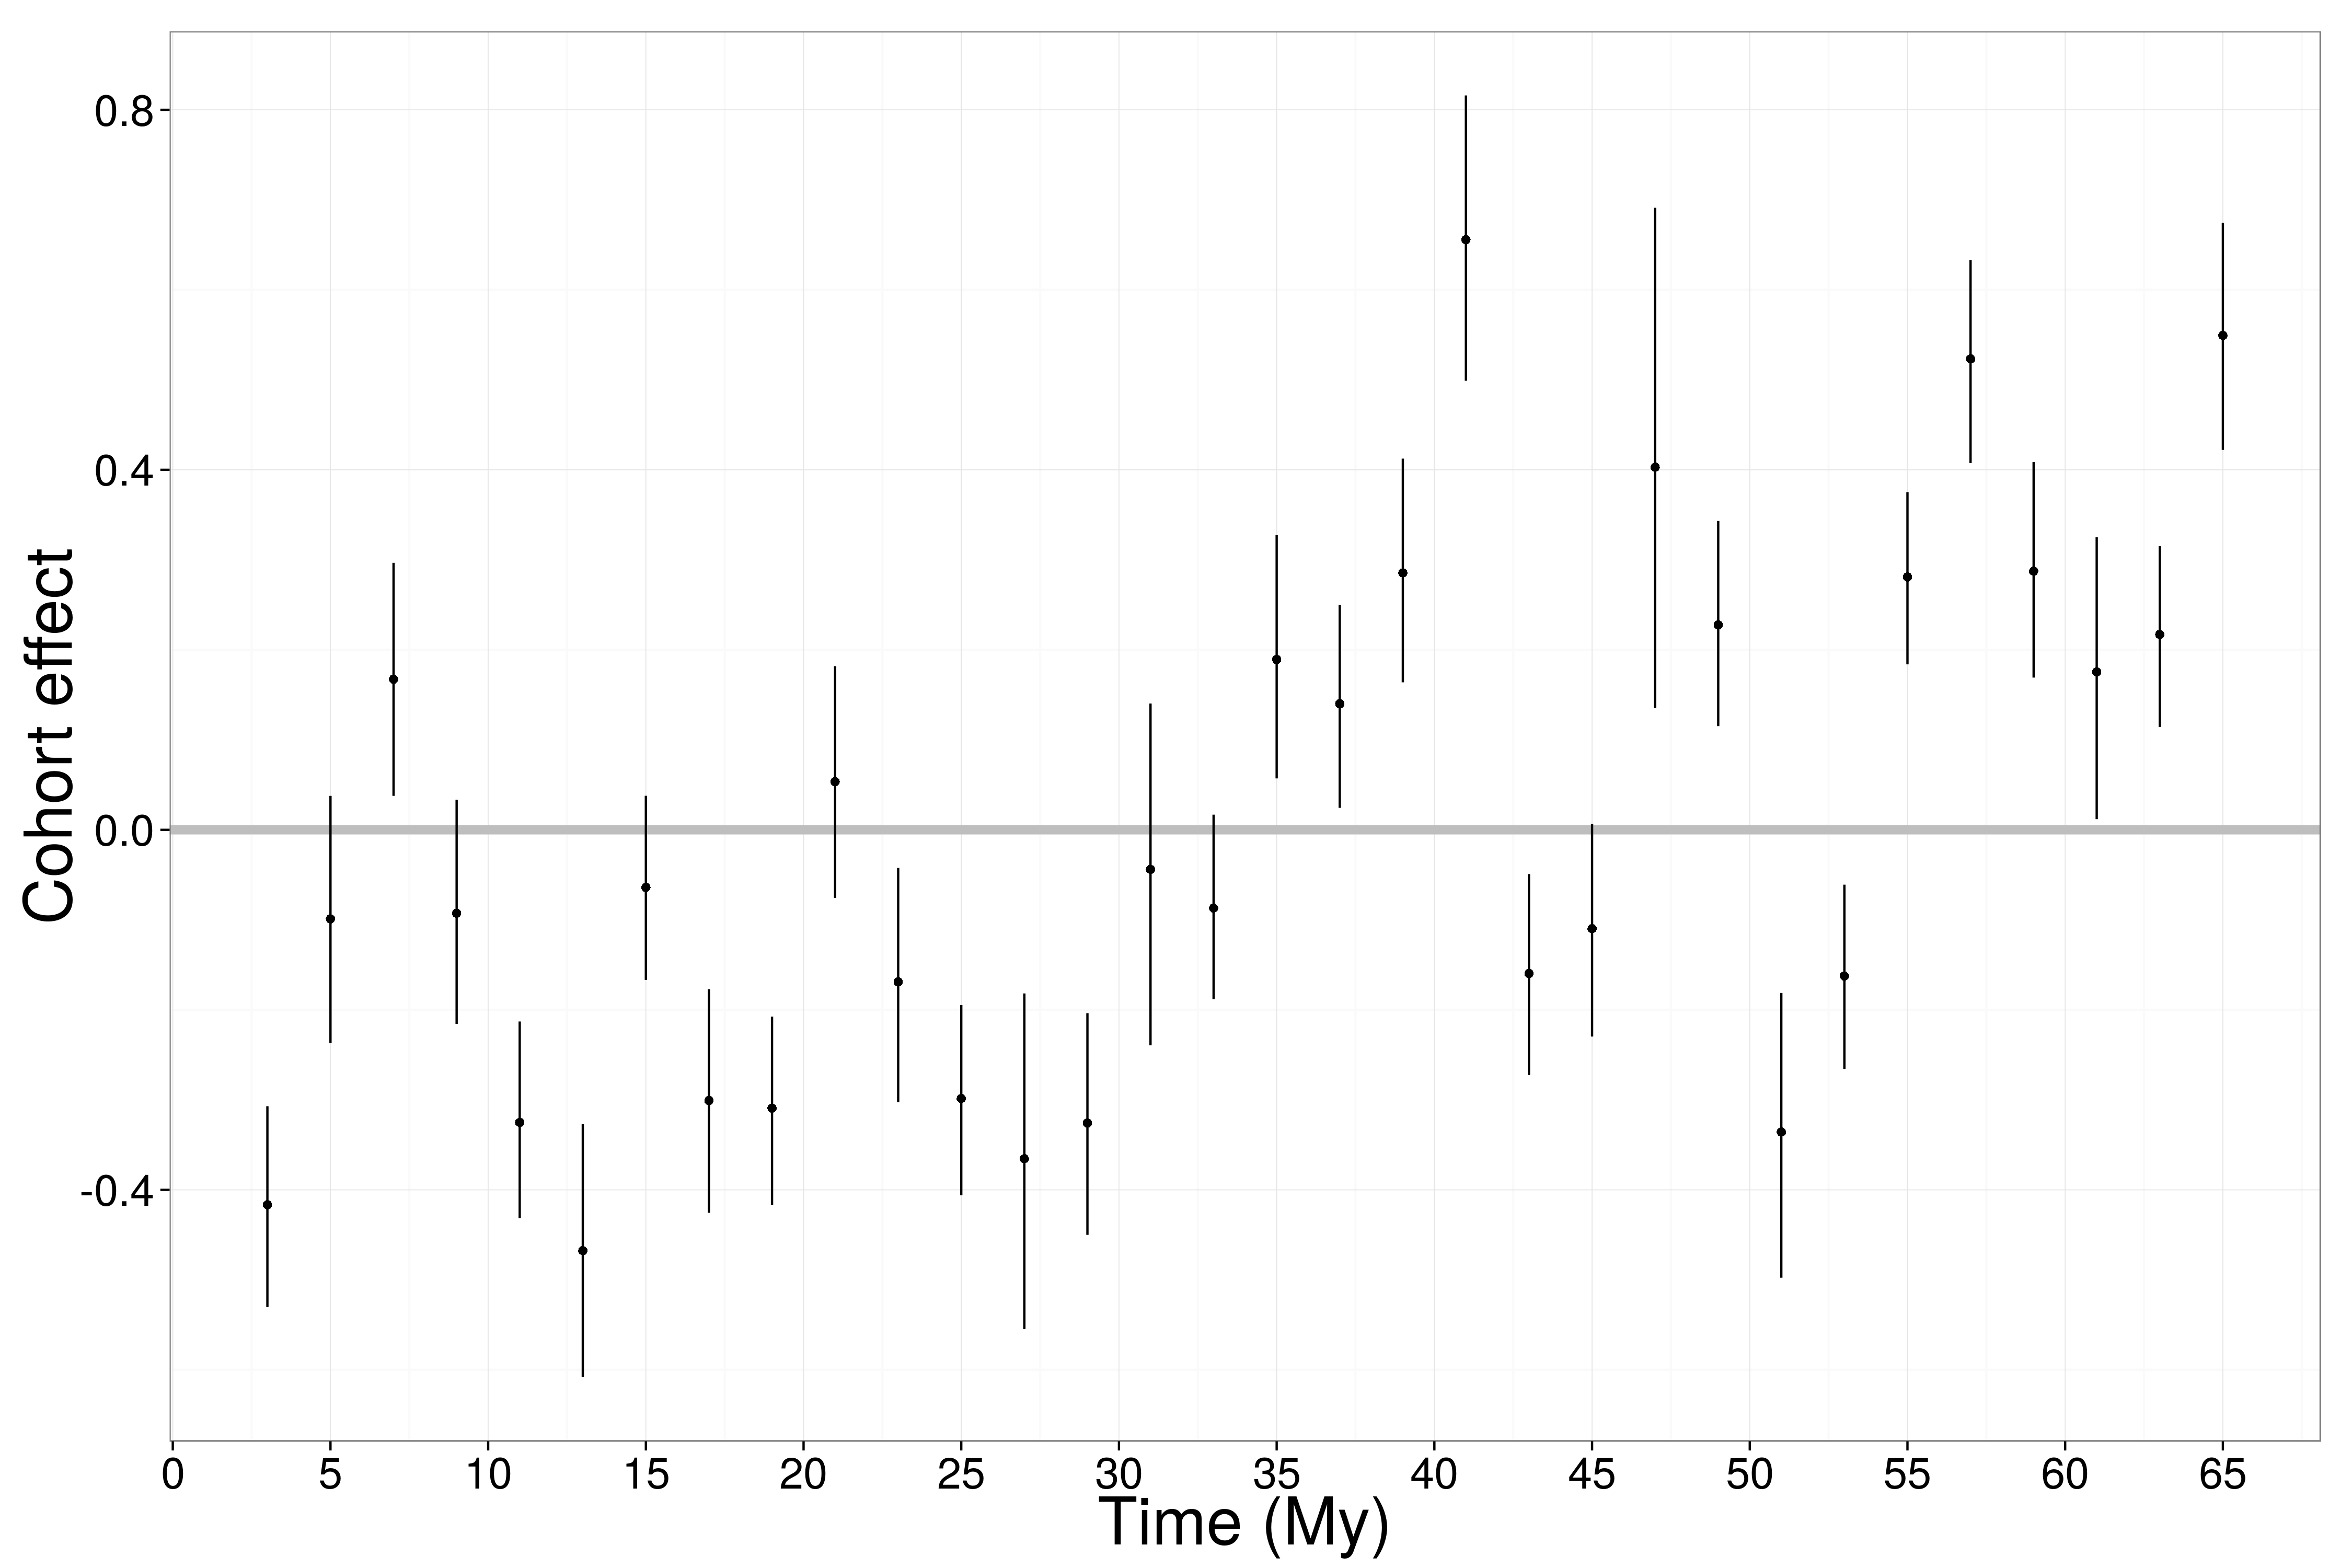
\includegraphics[height = 0.5\textheight, width = \textwidth, keepaspectratio = true]{figure/cohort_est}
  \caption{Summaries of estimated individual cohort effect posteriors. Depicted are medians and 80\% credible intervals of the estimated posterior distributions. High values correspond to shorter species durations while lower values correspond to greater species durations compared to the mean duration. Lines are placed at the middle of the 2 My origination cohorts.}
  \label{fig:eff_cohort}
\end{figure}

\begin{figure}[ht]
  \centering
  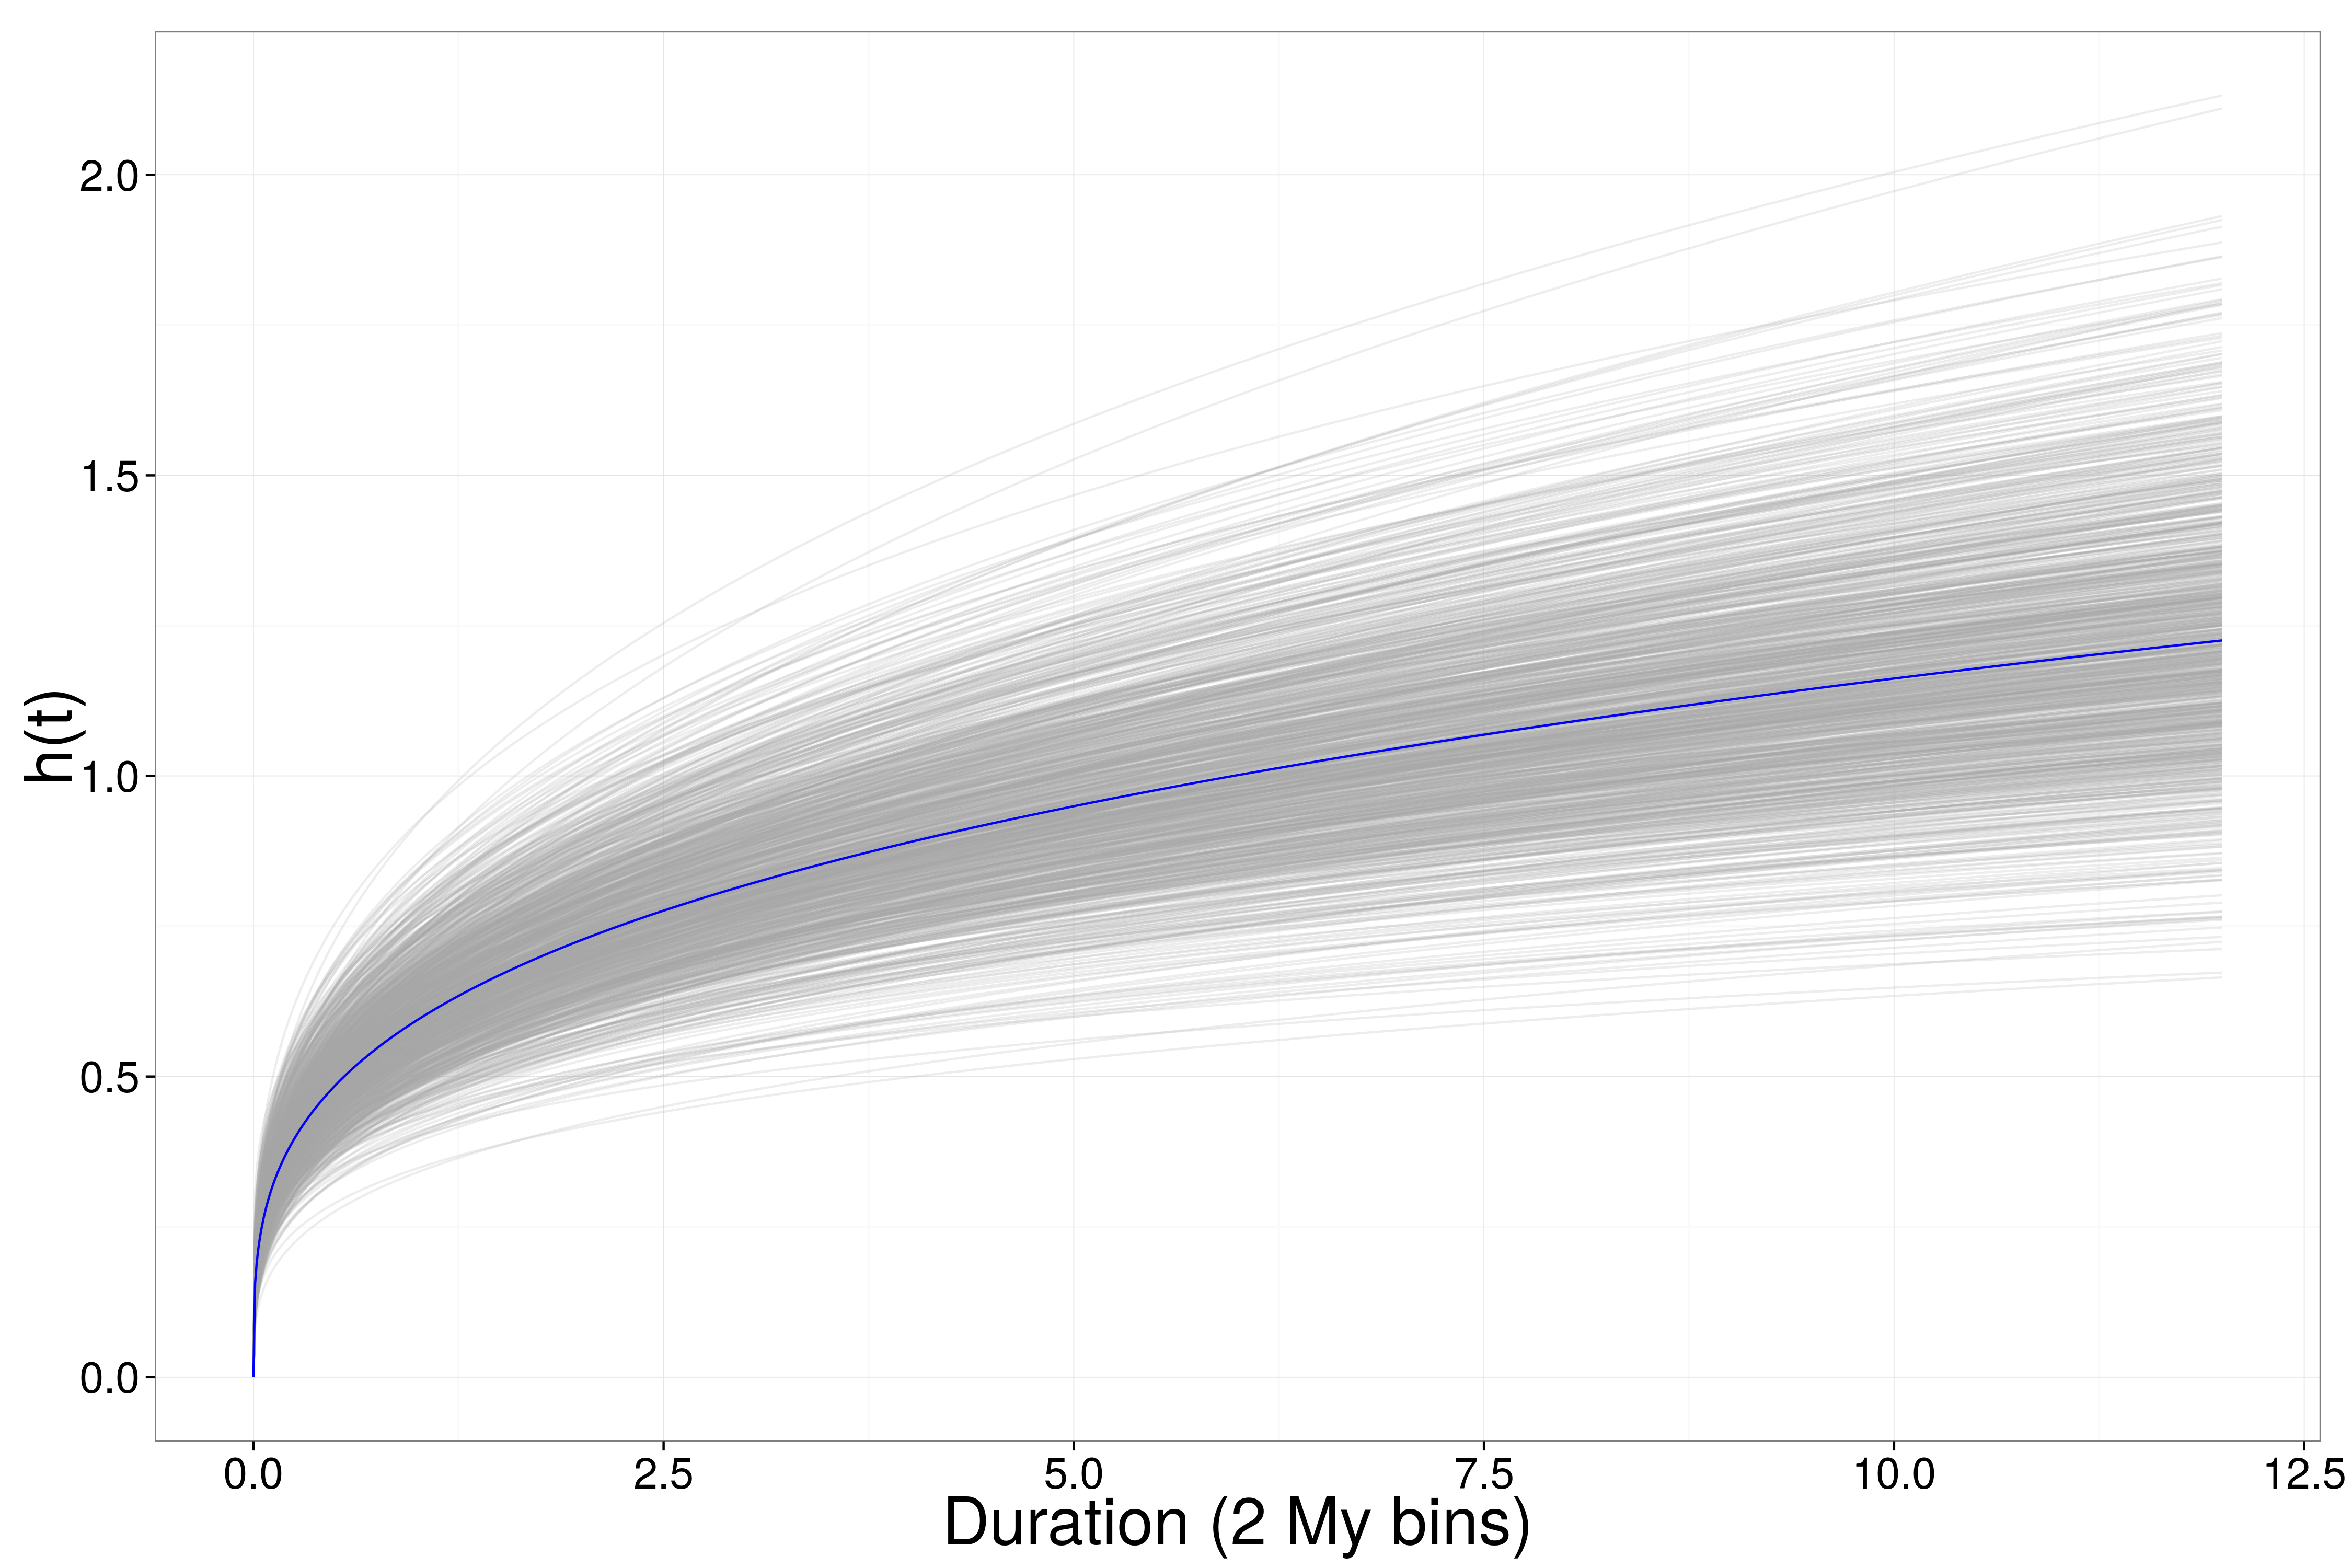
\includegraphics[height = 0.5\textheight, width = \textwidth, keepaspectratio = true]{figure/haz_est}
  \caption{100 estimates of the hazard function (\(h(t\)) for the observed species mean (grey), along with the median estimated hazard function. \(h(t)\) is an estimate of the rate at which a species of age \(t\) is expected to go extinct. Hazard functions were estimated from random draws from the estimated posterior distributions and evaluated with all covariate information set to 0, which corresponds to the expected duration of the mean species.}
  \label{fig:haz}
\end{figure}

\begin{figure}[ht]
  \centering
  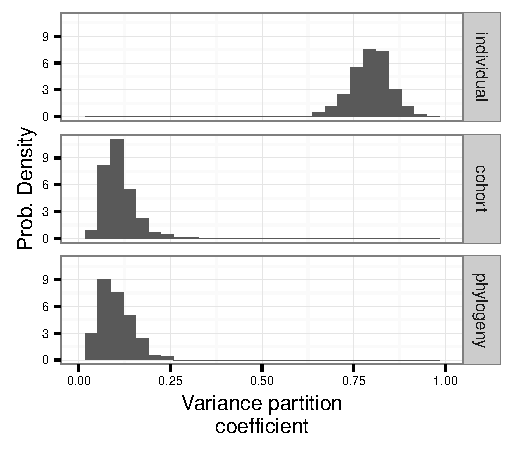
\includegraphics[height = 0.5\textheight, width = \textwidth, keepaspectratio = true]{figure/variance_est}
  \caption{Estimates of the variance partitioning coefficients for the three different sources of variance: species, cohort, and phylogeny. Higher values correspond to greater contribution to total observed variance. Each of the estimates is a distribution of 1000 approximating simulations due to the model's non-normality.}
  \label{fig:vpc}
\end{figure}

\end{document}
